\documentclass[12pt]{article}

\usepackage[utf8]{inputenc}
\usepackage[T2A]{fontenc}
\usepackage[english, russian]{babel}
\usepackage[a4paper, includefoot, left=1.5cm, right=1.5cm, top=1cm, bottom=1.5cm, headsep=1cm, footskip=1cm]{geometry}
\usepackage{makecell}
\usepackage{amsmath}
\usepackage{graphicx}
\usepackage{enumitem}
\usepackage{multirow}
\usepackage{hyperref}
\usepackage{mathtools}
\usepackage{amssymb}
\usepackage{textcomp}
\usepackage{booktabs}
\usepackage{float}

\begin{document}
\begin{large}
\begin{center}
\LARGE \textbf{Физика релятивистских звёзд}
\par
\LARGE \textbf{Кононов Александр Михайлович}
\par
\textbf{03.04.2026}
\end{center}

\par \textbf{Задача}:
\par Рассчитать зависимость радиуса от массы и температуры $R(M,T)$ для белого карлика из углерода с учётом кулоновских и тепловых поправок к уравнению состояния.

\par \textbf{Постановка модели}:
\par Рассматривается углеродный белый карлик, для которого
\[
A=12,\qquad Z=6,\qquad \mu_e=\frac{A}{Z}=2.
\]
В работе решалась ньютоновская система уравнений гидростатического равновесия
\[
\frac{dm}{dr} = 4\pi r^2 \rho,
\qquad
\frac{dP}{dr} = -\frac{Gm\rho}{r^2},
\]
где давление задаётся уравнением состояния
\[
P(\rho,T)=P_{e,0}(\rho)+P_{\mathrm{ion}}(\rho,T)+P_C(\rho).
\]

\par Основной вклад в давление даёт вырожденный электронный газ при $T=0$:
\[
P_{e,0}(x)=
\frac{\pi m_e^4 c^5}{3h^3}
\left[
x(2x^2-3)\sqrt{1+x^2}+3\,\mathrm{arsinh}\,x
\right],
\]
где
\[
x=\frac{p_F}{m_ec},
\qquad
p_F=\hbar(3\pi^2 n_e)^{1/3},
\qquad
n_e=\frac{\rho}{\mu_e m_u}.
\]

\par Тепловая поправка учитывалась в виде идеального давления ионов:
\[
P_{\mathrm{ion}}=\frac{\rho k_B T}{A m_u}.
\]

\par Кулоновская поправка бралась в приближении однородной ионной решётки:
\[
P_C=
-\frac{0.9}{3}
\left(\frac{4\pi}{3}\right)^{1/3}
Z^2 e^2 n_i^{4/3},
\qquad
n_i=\frac{\rho}{A m_u}.
\]

\par Таким образом, положительная тепловая добавка слегка увеличивает радиус, а отрицательная кулоновская поправка уменьшает радиус и массу при одной и той же центральной плотности.

\par \textbf{Расчет}:
\par Для каждого значения температуры выбиралась сетка центральных плотностей $\rho_c$. Далее система интегрировалась от центра к поверхности, где давление опускалось до малого порогового значения.
%Для ускорения вычислений уравнение состояния было предварительно табулировано на логарифмической сетке по плотности, а затем использовалась интерполяция $P(\rho)$ и обратной зависимости $\rho(P)$.

\par \textbf{Результаты}:

\begin{figure}[H]
    \centering
    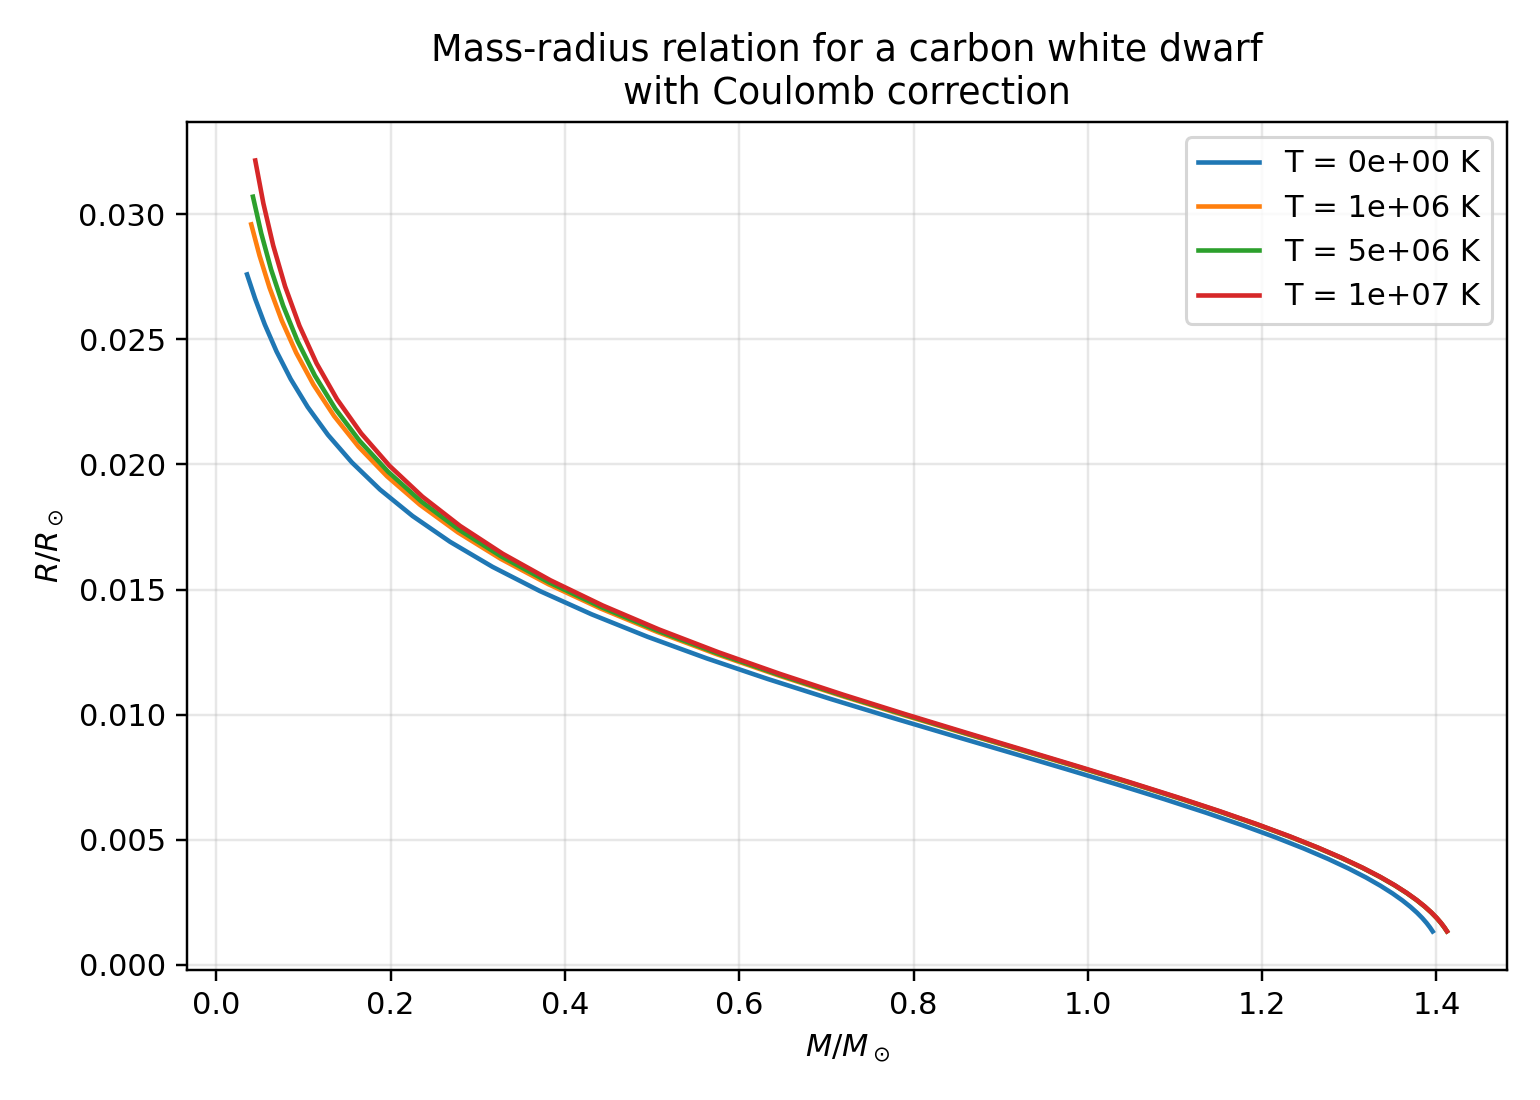
\includegraphics[width=0.82\textwidth]{mass_radius_temperatures.png}
    \caption{Зависимость $R(M)$ для разных температур при наличии кулоновской поправки.}
\end{figure}

На первом графике видно, что при фиксированной массе рост температуры ведёт к небольшому увеличению радиуса. Эффект особенно заметен у менее массивных белых карликов, где вклад теплового давления ионов относительно больше. Для массивных объектов, где давление почти полностью задаётся вырожденными электронами, температурная зависимость слабее.

\begin{figure}[H]
    \centering
    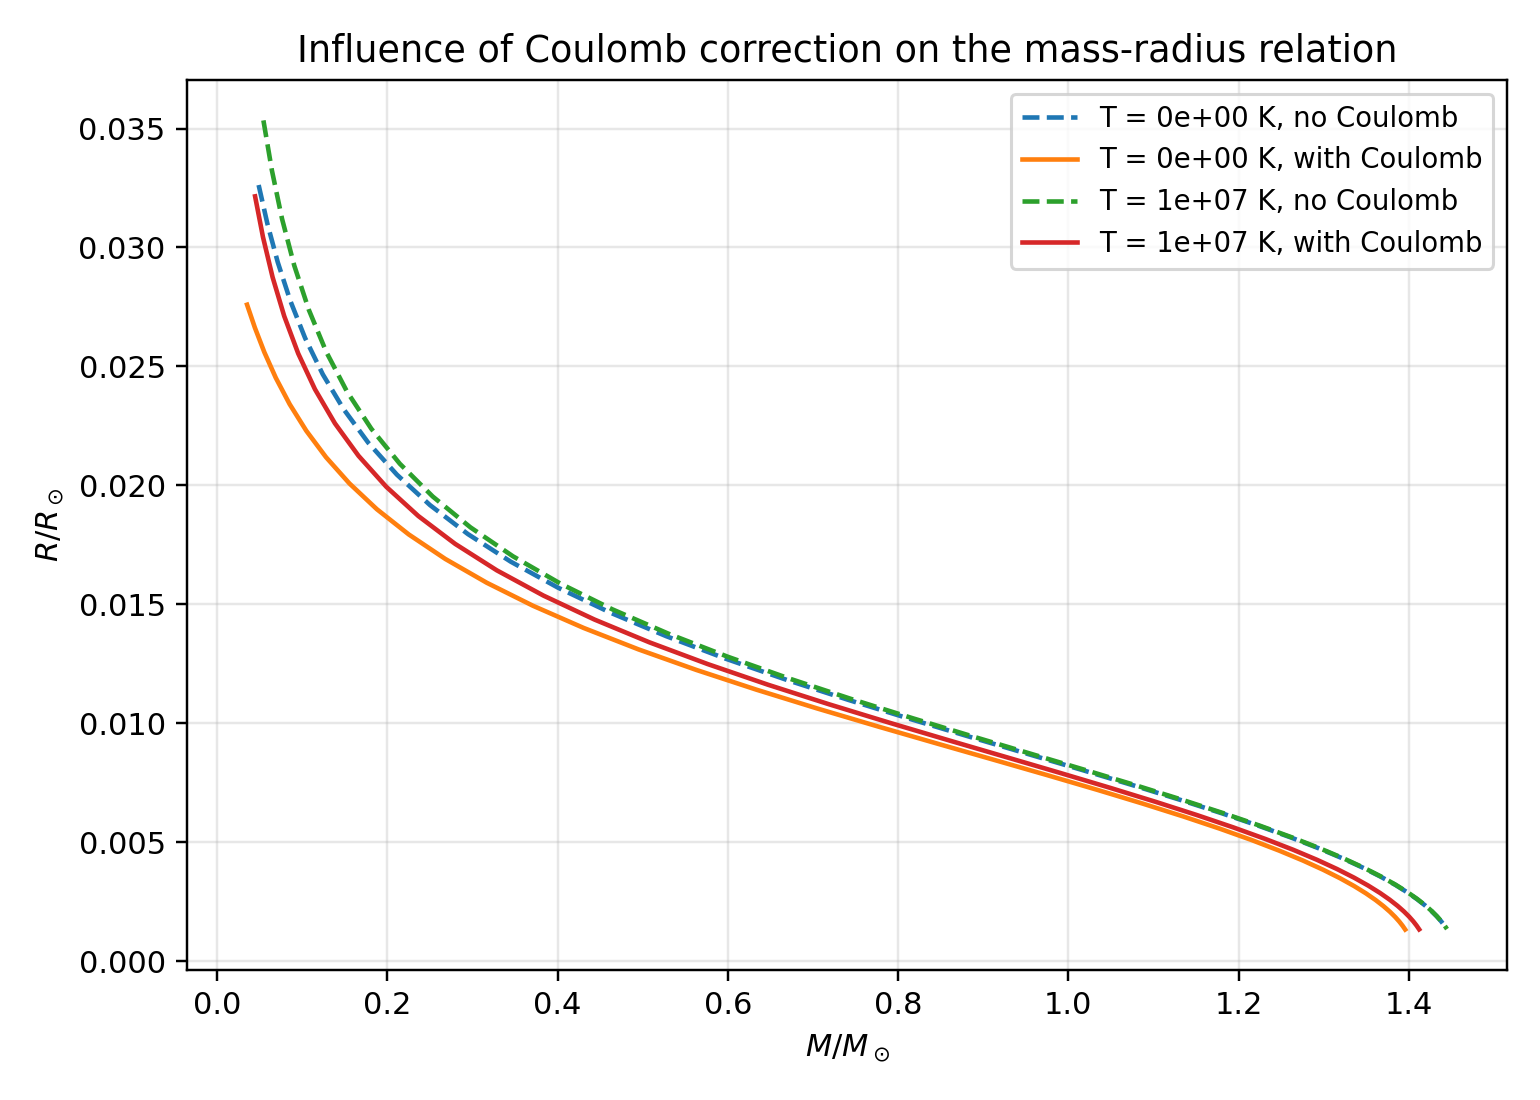
\includegraphics[width=0.82\textwidth]{mass_radius_coulomb.png}
    \caption{Сравнение кривых $R(M)$ с кулоновской поправкой и без неё.}
\end{figure}

Сравнение с моделью без кулоновской поправки показывает, что кулоновское взаимодействие делает звезду компактнее. Это физически ожидаемо: отрицательная кулоновская энергия уменьшает полное давление, поэтому для поддержания равновесия звезда должна сильнее сжаться.

\begin{figure}[H]
    \centering
    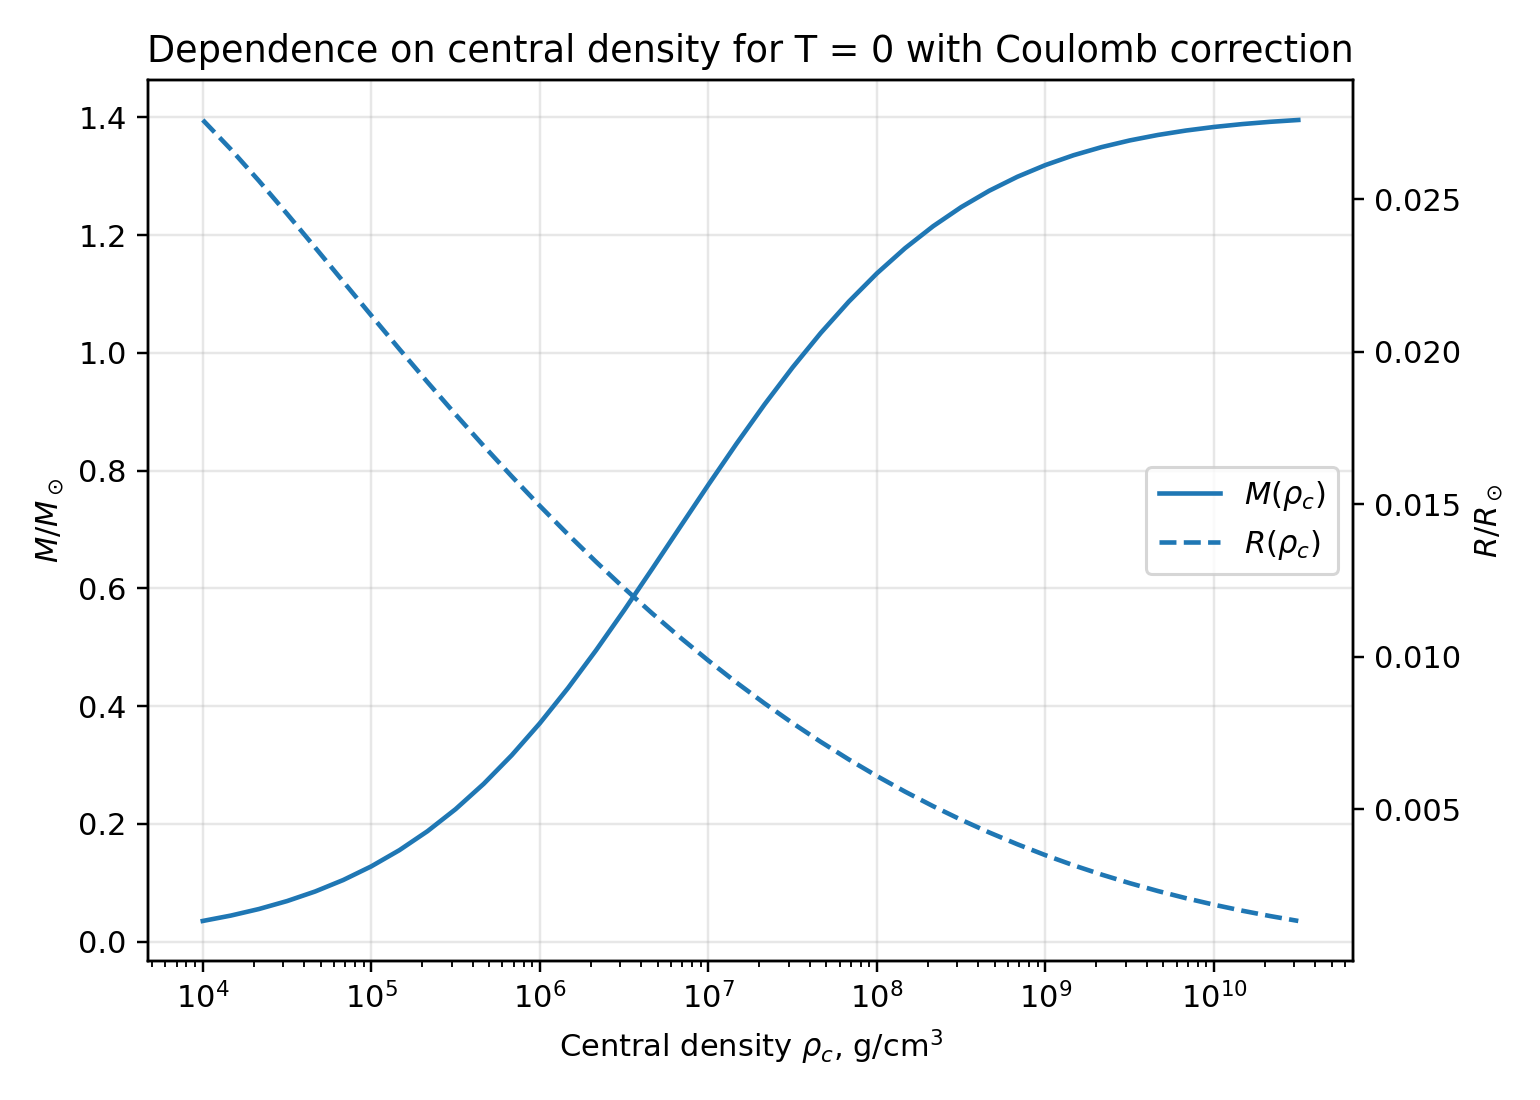
\includegraphics[width=0.82\textwidth]{central_density_dependence.png}
    \caption{Зависимость массы и радиуса от центральной плотности при $T=0$.}
\end{figure}

При увеличении центральной плотности радиус монотонно уменьшается, а масса сначала растёт и затем выходит на предельное значение порядка чандрасекаровской массы. В данной модели обратные бета-процессы не учитывались, поэтому формально кривая стремится к стандартному пределу, а не демонстрирует физическое уменьшение массы на сверхвысоких плотностях.

\begin{figure}[H]
    \centering
    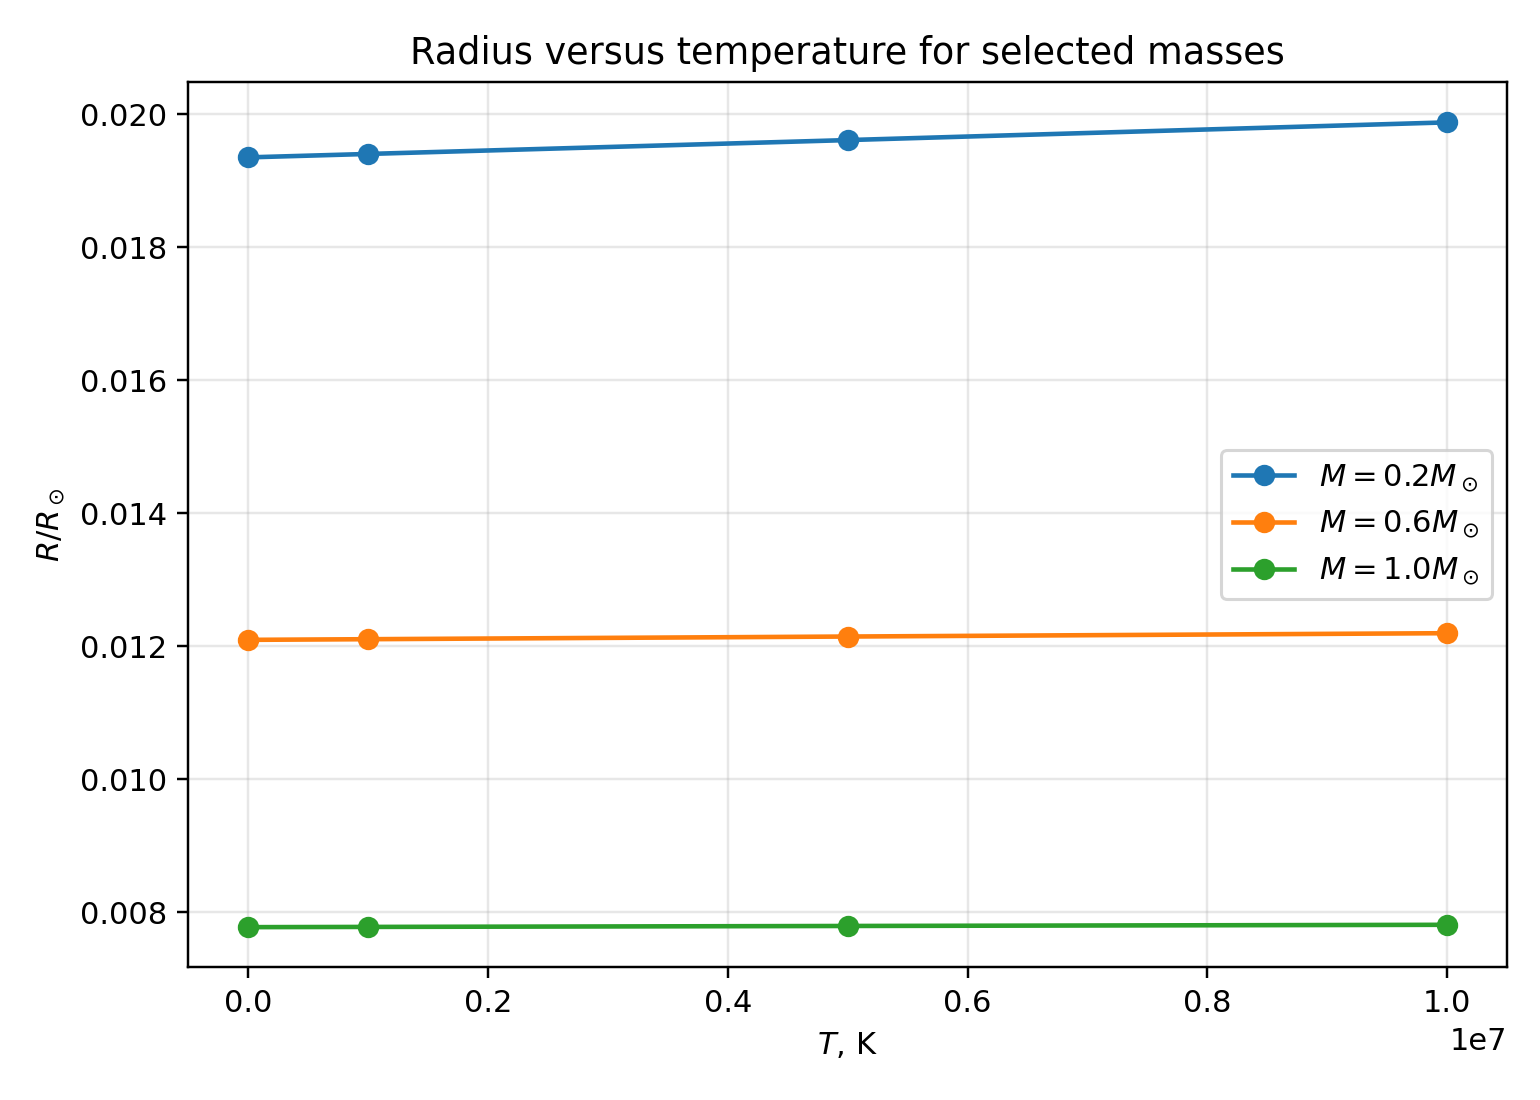
\includegraphics[width=0.82\textwidth]{radius_vs_temperature.png}
    \caption{Зависимость радиуса от температуры для нескольких фиксированных масс.}
\end{figure}

Этот график наглядно показывает, что при массе $1.0M_\odot$ температурная поправка практически не меняет радиус, тогда как для $0.2M_\odot$ увеличение температуры от $0$ до $10^7$ K приводит к уже заметному расширению.

\par \textbf{Сводная таблица}:

\begin{center}
\begin{tabular}{cccc}
\toprule
$T$, K & $M_{\max}/M_\odot$ & $R(M_{\max})/R_\odot$ & $\rho_c(M_{\max})$, г/см$^3$ \\
\midrule
0 & 1.412 & 0.0013 & 3.16e+10 \\
1e+06 & 1.412 & 0.0013 & 3.16e+10 \\
5e+06 & 1.412 & 0.0013 & 3.16e+10 \\
1e+07 & 1.412 & 0.0013 & 3.16e+10 \\
\bottomrule
\end{tabular}
\end{center}

%\par \textbf{Вывод}:
%\par В работе была построена численная зависимость $R(M,T)$ для углеродного белого карлика с учётом двух физических поправок к идеализированной модели: теплового давления ионов и кулоновского уменьшения давления. Полученные графики демонстрируют стандартное убывание радиуса с ростом массы, слабое температурное расширение при увеличении $T$ и дополнительное сжатие звезды при включении кулоновской поправки. Наиболее сильное влияние температура оказывает на маломассивные белые карлики, тогда как в области больших масс доминирует вырожденное электронное давление.

%\par Следует отметить, что данная модель описывает белый карлик как ньютоновскую звезду с конечной температурой и не включает обратный бета-распад, изменение химического состава и общерелятивистские эффекты. Поэтому результаты корректно интерпретировать как физически содержательную приближённую модель, пригодную для анализа влияния температуры и кулоновских поправок на зависимость $R(M,T)$.

\end{large}
\end{document}
